\documentclass[10pt,a4paper]{article}
\usepackage[utf8]{inputenc}
\usepackage{amsmath}
\usepackage{amsfonts}
\usepackage{amssymb}
\usepackage{graphicx}
\usepackage{url}
\usepackage{epstopdf}
\usepackage[ngerman]{babel}
\usepackage[ngerman]{translator}
\usepackage{listings}
\usepackage[singlelinecheck = false]{caption}
\usepackage[colorlinks=true,
        linkcolor=black,
        citecolor=black,
        filecolor=black,
        pagecolor=black,
        urlcolor=black,
        bookmarks=true,
        bookmarksopen=true,
        bookmarksopenlevel=3,
        plainpages=false,
        pdfpagelabels=true]{hyperref}

\parindent 0pt
\pagestyle{headings}

\let\oldsection\section
\renewcommand{\section}{\newpage \oldsection}

\title{
	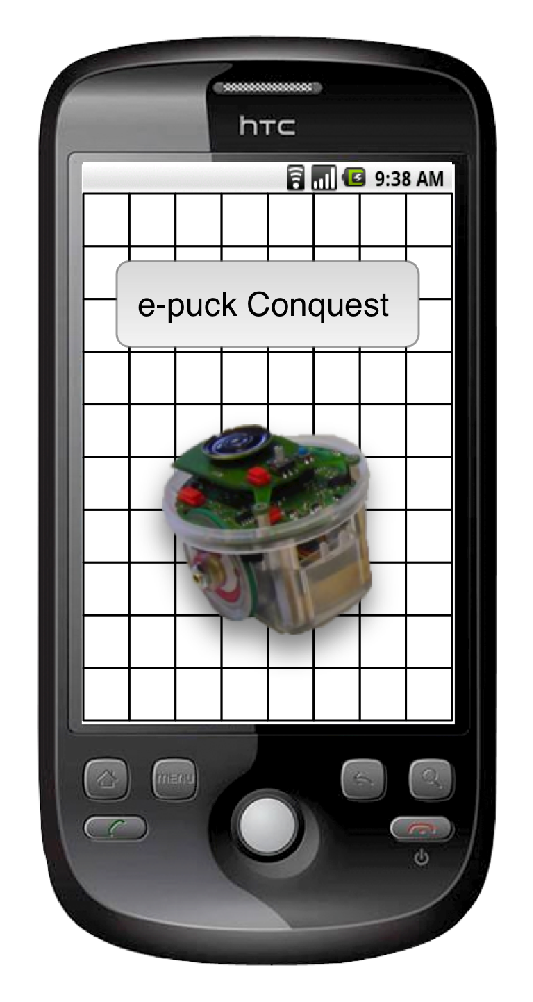
\includegraphics[height=10cm]{images/logo.eps} \\
	\vspace{1cm}
	Testbericht \\
	SEP-Conquest
}
\author{Andreas Wilhelm, Andreas Poxrucker, Martin Freund,\\ Max Binder, Florian B\"urchner, Florian Lorenz} 
\begin{document}
\date{14. Januar 2011}
	\maketitle
	\newpage
	\tableofcontents	
	\newpage
\section{Einleitung}
\section{Java-Testf\"alle mit JUnit}
	\subsection{GridMap}
	\begin{itemize}
		\item{testInsertNode} \\ F\"ugt einen Knoten in die Karte ein und \"uberpr\"uft die Anzahl der eingef\"ugten Objekte.
		\item{testFrontierNode} \\ F\"ugt zu jeweils einem Knotentypen einen Knoten ein und \"uberpr\"uft auf richtige FrontierNodes.
		\item{testUpdateNode} \\ F\"ugt nacheinander zwei benachbarte Knoten ein und \"uberpr\"uft ob der FrontierNode geupdatet wird.
		\item{testMapBorders} \\ F\"ugt in die Karte einige Knoten ein und \"uberpr\"uft auf die richtig gesetzten Grenzen des Feldes.
		\item{testSerializeMapInString} \\ Serialisiert eine Karte mit einigen Knoten in ein String-Array und \"uberpr\"uft auf richtiges Format.
	\end{itemize}
\section{C-Testf\"alle}
\section{Globale Testszenarien}
\end{document}